%-----------------------------------------------------
% Load packages for main document
%-----------------------------------------------------
\documentclass[12pt, a4paper,twoside,bibliography=totoc]{report} 	
\usepackage[ngerman]{babel} 	% Language English
\usepackage{lmodern}		 	% Latin Modern Fonts
\usepackage[T1]{fontenc}		% Schriften unterschiedlicher Kodierung
\usepackage[utf8]{inputenc}		% Eingabekodierung UTF8
\usepackage{listings}			% Listings Package
\usepackage{textcomp}			% Necessary for utf8 listings
\usepackage{paralist}			% Allows the usage of individual item-symbols
\usepackage{parskip} 			% Manages the space between sections, chapters, paragraphes
\usepackage{fancyhdr}			% Manages headers and footers
\usepackage{graphicx}			% Manages the import of pictures 
\usepackage{float}				% Allows the positioning of figures and tables on a fixed position
\usepackage{tabularx}			% Allows generation of long and wide tables
\usepackage{esdiff}				% Upright symbol when differentiating
\usepackage{amsmath}			% Allows the inclusion of formulas 
\usepackage{amssymb}			% Extends the variety of mathematical symbols
\usepackage{dsfont}				% Options for Mathematic Environment
\usepackage{hhline}				% Extends the possible lines in tables
\usepackage{longtable}			% Extends tabulars to be set on more than one page
\usepackage{tikz,pgfplots}				% Allows drawing vector graphics 
\usepackage{titlesec}			% Allows changing additional spaces between text and title
\usepackage{siunitx}			% Allows the usage of SI-symbols
\usepackage{pdfpages}			% Allows embedding pdf-pages 
\usepackage{epstopdf}			% Allows the usage of eps-figures 
\usepackage{titletoc} 			% Allows individual changes of the title page
\usepackage{lastpage}			% Allows writing X/Y where Y is document's last page
\usepackage{placeins}			% Allows separating of float environments
\usepackage{multirow}			% Allows combining several rows in tables
\usepackage{multicol}			% Allows combining several columns in tables
\usepackage{cite}				% Manages references and allows the embedding of BibTex
\usepackage[intoc]{nomencl}	    % Manages the nomenclature
\usepackage{lipsum}				% Allows the usage of lipsum-text
\usepackage{geometry}			% Allow the individual 
\usepackage{psfrag}
\usepackage{nicefrac}
\usepackage{caption}
\usepackage{graphicx,subcaption}
%\usepackage[demo]{graphicx}
\usepackage{colortbl}
\usepackage{listings}
\usepackage{hyperref}		%allows autoref



%-----------------------------------------------------
% Header and Footer
%-----------------------------------------------------
\fancyhf{} 			% clear all fields

\fancypagestyle{emptyPage}{%
	\fancyhead{}
	\fancyfoot{}
	\renewcommand{\footrulewidth}{0.0pt}
	\renewcommand{\headrulewidth}{0.0pt}
	\fancyheadoffset{0cm}
}%
\fancypagestyle{prolog}{%
	\fancyhead{}
	\fancyfoot{}
	\fancyfoot[C]{\textbf{\thepage}}
	\renewcommand{\footrulewidth}{0.8pt}
	\renewcommand{\headrulewidth}{0.0pt}
	\fancyheadoffset{0cm}
}%
\fancypagestyle{mainDocument}{%
	\fancyhead{}
	\fancyhead[RO]{\rightmark}
	\fancyhead[LE]{\leftmark}
	\fancyfoot{}
	\fancyfoot[RO,LE]{\textbf{\thepage}}
	\renewcommand{\footrulewidth}{0.8pt}
	\renewcommand{\headrulewidth}{0.8pt}
	\fancyheadoffset{0cm}
}%



%-----------------------------------------------------
% Configure nomenclature
%-----------------------------------------------------
\makenomenclature

%-----------------------------------------------------
% Configure Table of contents and Bibliography
%-----------------------------------------------------
\addto{\captionsenglish}{\renewcommand{\contentsname}{Table of contents}}
\addto{\captionsenglish}{\renewcommand{\bibname}{References}}

\begin{document}
	 
	%-----------------------------------------------------
	% Include cover sheet
	%-----------------------------------------------------	
	\include{01_Coversheet/coversheet}
	%-----------------------------------------------------
	% Change pagestyle and page layout
	%-----------------------------------------------------
	\newgeometry{includeheadfoot, bindingoffset = 25mm, 
		left = 5mm, 
		right = 20mm,
		headheight = 15mm,
		headsep = 8mm,
		textheight = 230mm,
		footskip = 16mm}
	%-----------------------------------------------------
	% Reset page counter and its style
	%-----------------------------------------------------	
	\pagestyle{fancy}	
	\setcounter{tocdepth}{2}
	\pagenumbering{Roman}
	\setcounter{page}{1}
	%-----------------------------------------------------
	% Preamble
	%-----------------------------------------------------
	%\section*{Foreword}
\thispagestyle{prolog}
\bigskip
\lipsum[1-3]


	
	%-----------------------------------------------------
	% Zusammenfassung
	%-----------------------------------------------------
	\section*{Aufgabenstellung}
\thispagestyle{prolog}
\bigskip

Für die Ansteuerung von elektrischen Maschinen wird oftmals eine Halbbrücke mit Bootstrapping-Schaltung verwendet. Die Aufgabe dieser Arbeit besteht darin, diese Art von Ansteuerung zu erklären. Es soll eine Transistorhalbbrücke mittels Bootstrap-Kondensator implementiert werden. Ebenso ist die \glqq Typical Application\grqq{} aus dem Datenblatt des LT1336 gegeben. Schlussendlich soll die Notwendigkeit der Aussteuerungsbegrenzung von Bootstrap-Schaltungen gezeigt werden. 
\hbox{ }

	%-----------------------------------------------------
	% Abstract
	%-----------------------------------------------------
	%\section*{Abstract}
\thispagestyle{prolog}
\bigskip

The goal of my bachelor's thesis is the automated evaluation of measurement data of a Force/Torque Sensor. A graphical user interface was created to make it easy for the user to work with its data. The Force Sensor is connected to a beared engine and this allows to get its Forces and Torques. Another task of my work was to implement some optional functions which the user can use - to save the data automated in Excel, for example.

Before programing, a literature research about the used Force Sensor was done, to get the know-how, how the Software should look for a easy use.

In the end the program was tested on an engine to guarantee a good working Software.

This work is a perfect mechatronic task. In addition to the measuring structure, it also includes software development as well as the connection to electrical machines.
\hbox{ }
\clearpage
	%-----------------------------------------------------
	% Table of contents
	%-----------------------------------------------------
	\tableofcontents
	\thispagestyle{prolog}
	\pagestyle{prolog}
	%-----------------------------------------------------
	\newpage 
	\setcounter{page}{1}
	\pagenumbering{arabic}
	\thispagestyle{mainDocument}
	\pagestyle{mainDocument}
	%-----------------------------------------------------
	% Chapter 1
	%-----------------------------------------------------
	%\include{06_Chapter1/chapter1}
	%-----------------------------------------------------
	% Chapter 2
	%-----------------------------------------------------
	%=====================================================
\chapter{Schaltungsprinzip}
\thispagestyle{mainDocument}
\pagestyle{mainDocument}
\label{chap_2}
%=====================================================
\begin{quote}
	Die Ansteuerung einer elektrischen Maschine (beispielsweise ein permanent erregter Gleichstrommotor) soll im Allgemeinen so ausgelegt werden, dass ein Betrieb in Vorwärts- und Rückwärtsrichtung gewährleistet werden kann. Daneben soll auch ein Bremsvorgang möglich sein, um dadurch eine Rückspeisung der Energie zu erzielen. Um die Ansteuerung mittels Transistorhalbbrücke einfacher zu verstehen wird nun kurz näher auf die Problematik eingegangen.
\end{quote}	
%=====================================================

%-----------------------------------------------------

%\subsection{This is a subsection}
%\label{subsec_2_1_1}
%-----------------------------------------------------
\section{Motivation}
\label{sec_2_2}

%-----------------------------------------------------
Aus dem Ersatzschaltbild einer elektrischen Maschine geht hervor, dass diese elektrisch gesehen (und sehr vereinfacht) aus einem Widerstand und einer Spule besteht. Vor allem diese Induktivität bildet die Grundlage für weitere Überlegungen. Die Ansteuerung eines Motors kann mittels einer Batterie und dem Schließen eines einfachen Schalters erfolgen (siehe Abbildung 1.1).
\begin{figure}[H]
	\renewcommand{\figurename}{Abbildung}
	\centering	
	\psfragscanon		
	\psfrag{P}[c][c]{$\hat{P}$}
	\includegraphics[width=0.8\textwidth,angle=0]{Bilder/1.jpg}		
	\caption{Aufbau zur Motoransteuerung.}
	\label{ME}
\end{figure}
\newpage
Bei geschlossenem Schalter fließt nun ein Strom in eingezeichneter Richtung (Abbildung 1.2) und die Maschine dreht sich, je nach Quellenspannung, mit maximaler Drehzahl. Um die Drehzahl steuern bzw. regeln zu können wird der Schalter mittels einer Pulsweitenmodulation (PWM) angesteuert. Dadurch wird erreicht, dass durch den Tastgrad, der mittlere Motorstrom eingestellt werden kann. 
 

\begin{figure}[H]
	\renewcommand{\figurename}{Abbildung}
	\centering	
	\psfragscanon		
	\psfrag{P}[c][c]{$\hat{P}$}
	\includegraphics[width=0.7\textwidth,angle=0]{Bilder/2.jpg}		
	\caption{Stromrichtung bei geschlossenem Schalter.}
	\label{ME}
\end{figure}

Interessanter wird es nach dem erneuten Öffnen des Schalters. Der Motor besteht im wesentlichen aus einer Induktivität. Die elektrischer Spule möchte aber nun trotzdem dafür Sorgen, dass der Strom weiterfließt. Für die Gewährleistung eines Stromkreislaufs sorgt nun die eingezeichnete Diode (Freilaufdiode).

\begin{figure}[H]
	\renewcommand{\figurename}{Abbildung}
	\centering	
	\psfragscanon		
	\psfrag{P}[c][c]{$\hat{P}$}
	\includegraphics[width=0.6\textwidth,angle=0]{Bilder/3.jpg}		
	\caption{Stromrichtung im Freilaufkreis.}
	\label{ME}
\end{figure}
\newpage
Die Problematik ergibt sich erst beim Bremsvorgang. In diesem Betriebsmodus wird der Motor zum Generator. Es erfolgt also eine Rückspeisung der Energie und der Stromfluss kehrt um. Beim geschlossenem Schalter funktioniert das noch ganz gut denn der Strom kann in die umgekehrte Richtung fließen. Beim öffnen des Stromkreislaufs muss sich der Strom jedoch einen anderen Weg suchen. Dieses mal kann dieser aber  nicht an der Diode vorbei. Diese ist nun in Sperrrichtung gepolt. Was folgt ist ein unkontrolliertes Ansteigen der Spannung im Motor, verursacht durch die unzufriedene Induktivität.

Nun liegt der Vorschlag nahe, die Diode mit einem zweiten Schalter zu ersetzen. Hierfür muss aber gesorgt werden, dass es nicht möglich ist beide Schalter zur gleichen Zeit zu schließen (Kurzschluss!). Mit dieser Schaltung ist es nun möglich, einen aktiven Bremsvorgang zu gewährleisten. Eine geregelte Drehrichtungsumkehr im Motorbetrieb kann aber damit noch immer nicht erfolgen. Die Schaltung muss erweitert werden.

\begin{figure}[H]
	\renewcommand{\figurename}{Abbildung}
	\centering	
	\psfragscanon		
	\psfrag{P}[c][c]{$\hat{P}$}
	\includegraphics[width=0.6\textwidth,angle=0]{Bilder/4.jpg}		
	\caption{Verschaltung als Vollbrücke.}
	\label{ME}
\end{figure}

Eine Schaltung wie in Abbildung 1.4 wird Vollbrücke genannt (Denkt man sich die rechte Hälfte weg erhält man die Halbbrücke wie vorhin). Sind die Schalter S1 und S4 geschlossen erhält man eine Drehrichtung wie vorhin. Durch die Ansteuerung von S2 und S3 kann nun ein Strom in die andere Richtung fließen und die Maschine dreht um. Auch der Bremsvorgang ist wieder möglich. Nun, da die Problematik im Prinzip geklärt wurde, kann auf die Auslegung der Schalter eingegangen werden.
\newpage
\section{Realisierung der Schaltung}
\label{Aufbau}

\label{sec_2_3}

Abbildung 1.5 zeigt eine mögliche Realisierung des besprochenem Konzepts. Für die Schalter kommen zwei n-Kanal Mosfets zum Einsatz (M3 und M4). Die Last (die Ersatzschaltung des Motors) bilden die Induktivität L1 und der Widerstand R8. Auch die Versorgung UBatt ist links oben mit 14\,V gewählt.

\begin{figure}[H]
	\renewcommand{\figurename}{Abbildung}
	\centering	
	\psfragscanon		
	\psfrag{P}[c][c]{$\hat{P}$}
	\includegraphics[width=1\textwidth,angle=0]{Bilder/6.jpg}		
	\caption{Halbbrückenansteuerung mit Bootstrap.}
	\label{ME}
\end{figure}

Die Grundlage für die Ansteuerung der beiden Mosfets sind die PWM-Signale V1 und V3. Um ein gleichzeitiges leiten der Fets zu verhindern, soll eine Totzeit gewählt werden (beispielsweise 1\,$\mu$s). Fürs erste betrachten wir nun die Lowside, also den unteren Teil der Schaltung. Für das Ansteuern ist es wichtig zu wissen, dass jeder Fet zwischen Gate und Source eine Kapazität darstellt. Diese muss beim Schalten sehr schnell umgeladen werden. Daneben wird auch ein hoher Spannungshub am Gate benötigt um den Fet zu schalten. Um dies zu erreichen gibt es vor dem eigentlichen Schalter zwei Stufen. Die erste besteht wieder aus einem n-Kanal Mosfet (M2) für sehr kleine Ströme und Spannungen, sowie dem Pullup-Widerstand R4. Durch diese Schaltung wird das PWM-Signal invertiert. Liegt am Eingang des Gates High an, wird der FET leitend und das Potenzial wird auf Ground gezogen. Ist das Signal jedoch auf Low, leitet der FET nicht und das Potenzial wird über R4 auf UBatt gezogen. Neben dieser Invertierung, wurde hier auch noch der benötigte hohe Spannungshub erreicht. Nun ergibt sich eine Spannung zwischen 0\,V und UBatt, angepassst an das PWM-Signal. 

Die zweite Problemstellung war, dass das Gate einen sehr hohen Strom in kurzer Zeit braucht. Dafür wird eine zweite Halbbrücke aus zwei Bipolartransistoren aufgebaut. Durch diese Verschaltung erreicht man sehr hohe Ströme in sehr kurzer Zeit.

Nun, da die Lowside ausgelegt wurde, können wir uns mit der Highside beschäftigen. Der Mosfet, welcher hier verwendet wurde ist ebenso wieder ein n-Kanal Typ. Prinzipiell kann auch ein p-Kanal Mosfet hier zum Einsatz kommen. Das würde den Vorteil mit sich bringen die selbe Schaltung wie in der Lowside aufbauen zu können. Diese Art von Fets werden aber in der Praxis nicht gerne verwendet, da der Kanalwiderstand im gesättigten Zustand deutlich höher ist als bei n-Kanal Fets. Diese Eigenschaft möchte man jedoch möglichst vermeiden und nimmt daher eine kompliziertere Ansteuerschaltung in Kauf. Auch hier, auf der Highside, soll die Gate-Source Spannung auf dem Potenzial von UBatt liegen. Das Problem: Source des M3 kann unter Umständen schon auf UBatt liegen. Das bedeutet, dass am Gatetreiber eine deutlich höhere Spannung anliegen muss, da ansonsten der Fet nicht schalten wird. Man könnte auch ein Netzteil verwenden, doch dies wäre für diese Anwendung eher aufwändig, da im Mittel nur kleine Ströme fließen  (Schaltströme sind nur kurzzeitig hoch). 

Jetzt kommt die schon erwähnte Bootstrap Schaltung zum Einsatz. Gehen wir davon aus, dass der untere Mosfet M4 leitet. Load, also die Last liegt auf Masse. Nun gilt 
\begin{equation}
	U_{BOOT}=U_{Batt}-U_{D1}.
\end{equation}
$\rightarrow$ Der Kondensator C1 lädt sich auf.

Wenn nun M4 sperrt möchte man, dass M3 leitet. Da nun UBootstrap ungefähr auf dem Potenzial von UBatt liegt, liegt auch am Gate des Highside Mosfets ungefähr UBatt an. Source liegt vorerst auf Masse, da dies vom sperrenden FET so vorgegeben wird. Im nächsten Moment liegt Source auf UBatt - genauso wie das Gate. Der noch geladene Kondensator C1 beginnt sich zu entladen und adddiert zu UBootstrap diese Spannung. Das ergibt zwei mal UBatt. Nun ist die Spannung groß genug um auch M3 schalten zu können. Für eine Drehrichtungsumkehr kann die Halbbrücke mit denselben Bauelementen am rechten Ende der Last nochmals ident aufgebaut werden. Dies ergäbe dann die schon erwähnte Vollbrücke.

\section{Deadtime-Simulation}
In diesem Abschnitt wird die minimalmögliche Totzeit ermittelt, sodass es zu keinem Kurzschluss kommt. Im Zuge dieser Analyse ist ein Stromimpuls aufgetaucht, welcher nicht durch Vergrößern der Totzeit reduziert werden konnte.
\subsection{Stromüberhöhung beim Einschalten}
Bei einer einfachen Halbbrücke ohne zusätzliche Diode parallel zu M4 wird beim Einschalten von M3 ein Kurzschluss verursacht, obwohl M4 bereits abgeschaltet ist und der Strom über die Body-Diode fließt. Schaltet M4 zu schnell ein kommt es zu einem Kurzschluss, weil die Body-Diode noch nicht sperrt.
Dieser Effekt kann durch zwei Maßnahmen reduziert werden:
\begin{itemize}
    \item Reduktion der Schaltgeschwindigkeit von M3 durch Vergrößerung des Gate-Widerstandes oder dem
    \item Einbau einer zusätzlichen Diode.
\end{itemize}
Um den Strompeak kleiner als den Maximalstrom zu bekommen muss der Gatevorwiderstand ca.$\SI{1000}{\ohm}$ sein, wodurch sich ein und Ausschaltzeiten wesentlich erhöhen. Aufrgrund dieser langsamen Schaltzeiten muss auch die Totzeit sehr groß sein. Daher ist dies keine zufriedenstellende Lösung für das Problem.
Durch den Einbau einer Diode vom Typ RBR40NS30A parallel zur Body-Diode kann dieses Problem vollständig eliminiert werden. Nach dem Ausschalten von M4 fließt der gesamte Strom über die Diode und es kommt zu keinem Kurzschluss. Deshalb wird in folgendem Abschnitt die zweite Variante genommen.
\begin{figure}
     \centering
     \begin{subfigure}[t]{0.33\textwidth}
         \centering
         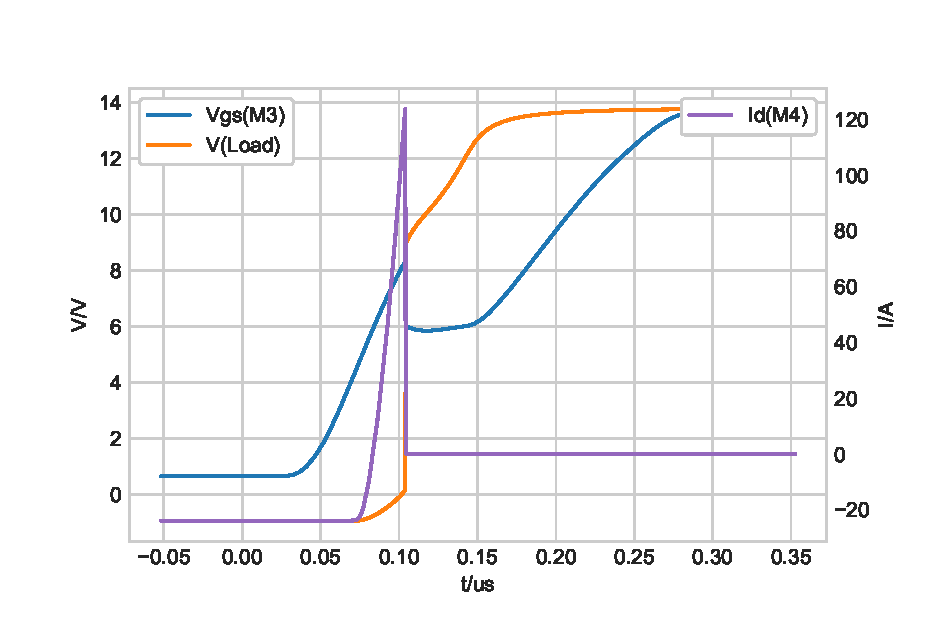
\includegraphics[width = \textwidth]{Bilder/NoDiode.eps}
         \caption{Keine Diode, kein Gatewiderstand}
     \end{subfigure}
     \begin{subfigure}[t]{0.33\textwidth}
         \centering
         \includegraphics[width = \textwidth]{Bilder/NoDiodeResistor.eps}
         \caption{Keine Diode, $\SI{1000}{\ohm}$ Gatewiderstand}
     \end{subfigure}
     \begin{subfigure}[t]{0.32\textwidth}
         \centering
         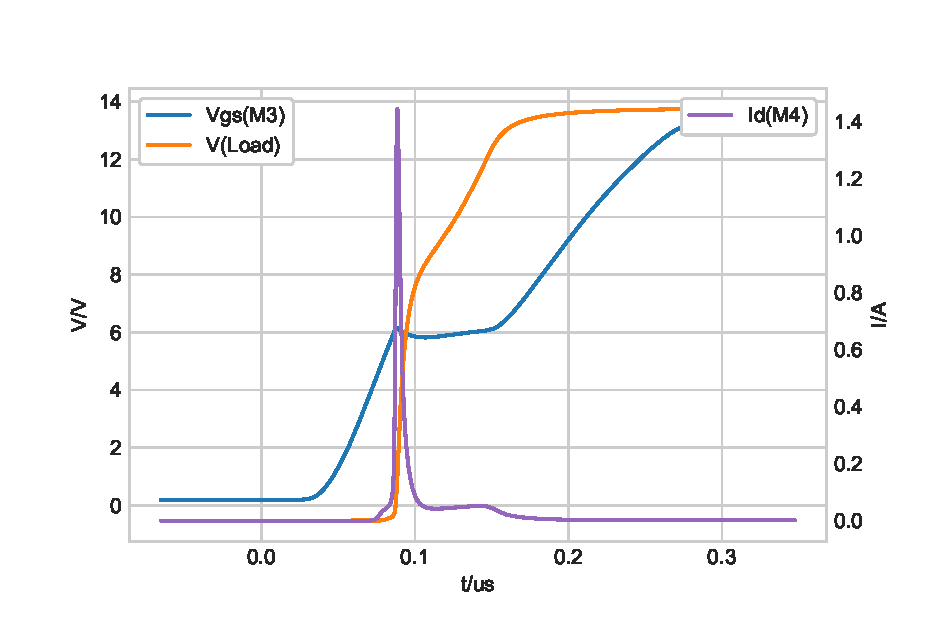
\includegraphics[width = \textwidth]{Bilder/Diode.eps}
         \caption{mit externer Diode}
     \end{subfigure}
        \caption{Vergleich der Spannungen und Ströme beim Einschaltvorgang.}
        \label{fig:three graphs}
\end{figure}
\subsection{Minimale Totzeit}
Um die minimale Totzeit zu bestimmen, wird eine Parametersimulation durchgeführt. Der Drainstrom von M4 ist im Idealfall immer gleich null. Sehr hohe positive Ströme können nur aufgrund eines Kurzschlusses fließen, daher ist das Maximum von \texttt{Id(M4)} ein Indikator für einen Kurzschluss. Das Ergebnis dieser Simulation ist in \autoref{fig:DeadtimeVariation} dargestellt. Die minimale Totzeit ist somit ca. $\SI{50}{ns}$.
\begin{figure}
    \centering
    \includegraphics[width=0.8\textwidth]{Bilder/DeadtimeStepped.eps}
    \caption{Maximalstrom im Transistor über die eingestellte Totzeit.}
    \label{fig:DeadtimeVariation}
\end{figure}

\section{Aussteuerbegrenzung}
Da der Bootstrap-Kondensator immer dann geladen wird, wenn M4 eingeschaltet ist, kann 100\% Tastgrad nie erreicht werden. Wird der Tastgrad nicht begrenzt, so bricht die Bootstrap-Spannung zusammen und M3 sättigt aufgrund der sinkenden Gate-Spannung.
Die maximale Tastgrad hängt vom Stromverbrauch der Ansteuerschaltung und von der Größe des verwendeten Kondensators ab.
\begin{figure}
    \centering
    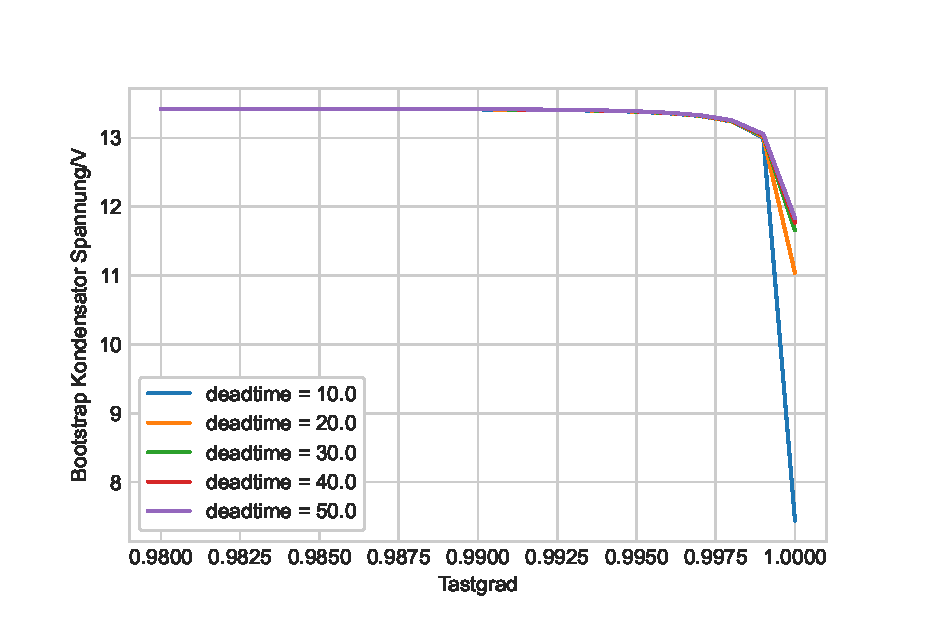
\includegraphics{Bilder/Aussteuerbegrenzung.eps}
    \caption{Mittlere Spannung am Bootstrap-Kondensator in Abhängigkeit vom Tastgrad und der eingestellten Totzeit.}
    \label{fig:Aussteuerbegrenzung}
\end{figure}
Wie in \autoref{fig:Aussteuerbegrenzung} zu sehen ist, hat auch die Totzeit einen Einfluss auf den maximalen Tastgrad, da selbst bei 100\% Aussteuerung die Totzeit verbleibt.


%======================================
\FloatBarrier
\clearpage
%=====================================================
	%-----------------------------------------------------
	% Chapter 3
	%-----------------------------------------------------
	%\include{08_Chapter3/chapter3}
	%-----------------------------------------------------
	% Chapter 4
	%-----------------------------------------------------
	%\include{09_Chapter4/chapter4}
	%%% Nomenclature
	%-----------------------------------------------------
	%\nomenclature{$\mu_0$}{permeability in vacuum}
	%-----------------------------------------------------
	%%%\printnomenclature
	\thispagestyle{mainDocument}
	\clearpage
	%-----------------------------------------------------
	% References
	%-----------------------------------------------------
	%\nocite{Zagar}
	%-----------------------------------------------------


	\addcontentsline{toc}{chapter}{Literaturverzeichnis}
	\clearpage
\end{document}
